\documentclass[../thesis.tex]{subfiles}

\begin{document}

% \begin{lstlisting}[style=code]
% Dương Lữ Điện
% \end{lstlisting}

Google Translate là một dịch vụ dịch thuật được phát triển bởi Google hỗ trợ trên 100 ngôn ngữ khác nhau. Số liệu thống kê vào tháng 05 năm 2013 cho thấy, Google Translate phục vụ dịch thuật cho hơn 200 triệu người mỗi ngày.

Google Cloud Translation API là một API thuộc nhóm Cloud Machine Learning API. Cloud Translation API cung cấp một giao diện lập trình ứng dụng đơn giản để lập trình viên có thể tích hợp tính năng phiên dịch (Translation) của Google vào website hoặc ứng dụng của họ. Với tính tương thích cao, các website và ứng dụng tích hợp Google Translation hoạt động rất hiệu quả trong việc phiên dịch từ một ngôn ngữ sang một ngôn ngữ khác (Ví dụ: từ tiếng Anh sang tiếng Việt). Ngoài ra, tính năng phát hiện ngôn ngữ cũng hoạt động khá hiệu quả khi ngôn ngữ gốc chưa được xác định.

Trong tài liệu này, chúng tôi sử dụng Google Cloud Translation API version 2 revision 51. Minh hoạ bằng ngôn ngữ lập trình Java. 

\section{Đăng ký sử dụng Google Cloud Platform}

Để truy cập đến các dịch vụ của Google Cloud Platform, ta sử dụng tài khoản Google. Để nhận \$300 credit dùng thử trong 1 năm từ Google, ta truy cập vào link:
\begin{lstlisting}[style=link]
https://console.cloud.google.com/freetrial
\end{lstlisting}
và điền đầy đủ các thông tin mà Google yêu cầu, bao gồm cả thông tin thẻ tín dụng (Hình \ref{Dien day du thong tin ma Google yeu cau} và \ref{Thong bao cua Google khi dang ky thanh cong}).

\begin{figure}
	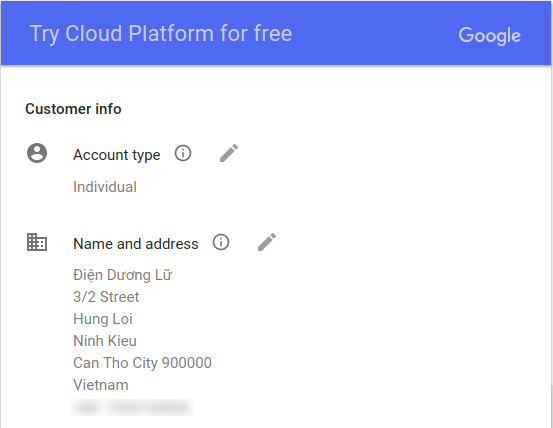
\includegraphics[width=\textwidth, keepaspectratio]{trial-2.png}
	\caption{Điền đầy đủ thông tin Google yêu cầu}
	\label{Dien day du thong tin ma Google yeu cau}
\end{figure}

\begin{figure}
	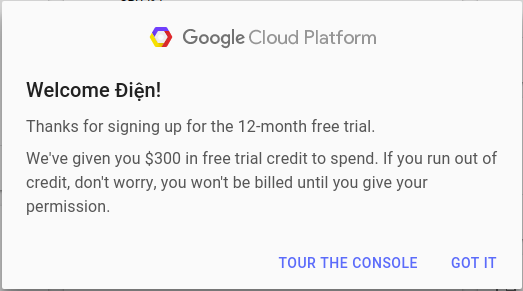
\includegraphics[width=\textwidth, keepaspectratio]{trial-4.png}
	\caption{Thông báo của Google khi đăng ký thành công}
	\label{Thong bao cua Google khi dang ky thanh cong}
\end{figure}

\section{Tạo một project trên Google API Console}

\begin{enumerate}
	\item Truy cập vào Google Cloud Platform Console.
	\begin{item}
	Tạo một project tên là ``translation'' (Hình \ref{Tao mot project tren Google Cloud Platform}).
	\begin{figure}
		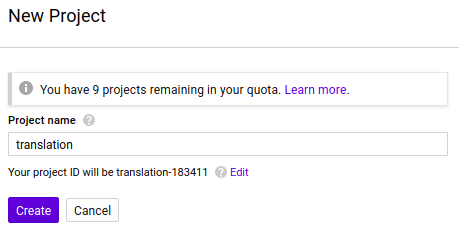
\includegraphics[width=\textwidth, keepaspectratio]{create-project.png}
		\caption{Tạo một project trên Google Cloud Platform}
		\label{Tao mot project tren Google Cloud Platform}
	\end{figure}
	\end{item}
\end{enumerate}

\section{Kích hoạt Google Cloud Translation API}
\begin{enumerate}
	\item Từ thanh tìm kiếm, nhập từ khoá ``Google Cloud Translation API''.
	\begin{item}
	Nhấp vào nút ``Enable'' để kích hoạt dịch vụ Translation (Hình \ref{Kich hoat dich vu Translation}).
	\begin{figure}
		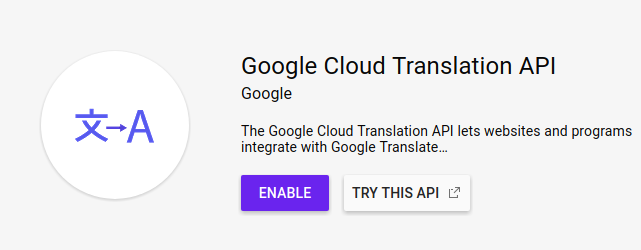
\includegraphics[width=\textwidth, keepaspectratio]{enable.png}
		\caption{Kích hoạt dịch vụ Translation}
		\label{Kich hoat dich vu Translation}
	\end{figure}
	\end{item}
\end{enumerate}

\section{API key}

API key là một chuỗi được mã hoá nhằm giúp cho Google nhận định danh được người dùng đang sử dụng dịch vụ, tính toán băng thông và tính phí dịch vụ. Để lấy API key cho ứng dụng, ta thực hiện các bước sau:

\begin{enumerate}
	\item Từ Google Cloud Platform Console menu, vào APIs and services > Credentials.
	\item Tạo một API key và tiến hành hạn chế quyền truy cập đến API key này.
\end{enumerate}

\section{Tạo một project trên Eclipse}
\begin{enumerate}
	\item Cài đặt gói M2Eclipse.
	\begin{item}
	Vào File > New > Other\ldots > Maven > Maven Project (Hình \ref{Tao mot project Maven tren Eclipse} và \ref{Thiet lap Archetype Parameters}).
	\begin{figure}
		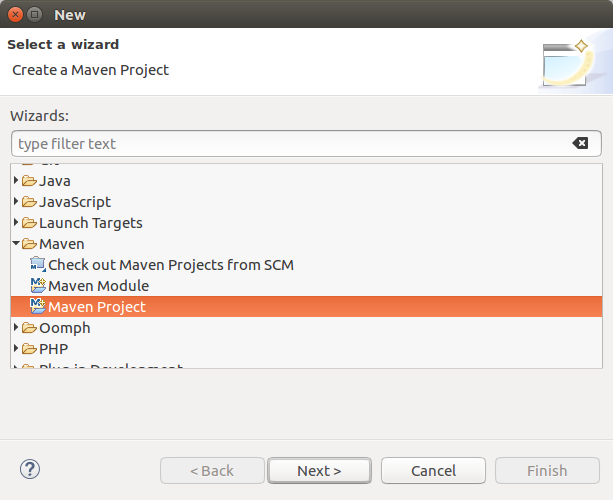
\includegraphics[width=\textwidth, keepaspectratio]{create-maven-project-1.png}
		\caption{Tạo một project Maven trên Eclipse}
		\label{Tao mot project Maven tren Eclipse}
	\end{figure}
	\begin{figure}
		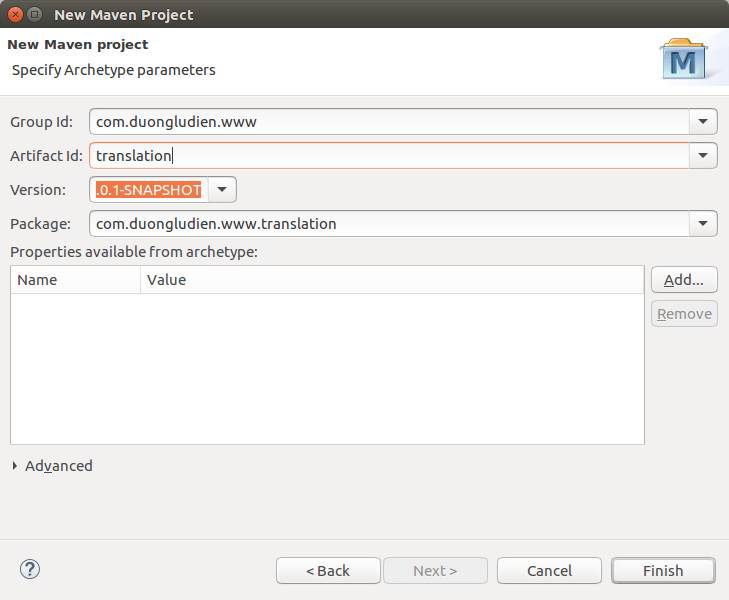
\includegraphics[width=\textwidth, keepaspectratio]{create-maven-project-2.png}
		\caption{Thiết lập Archetype Parameters}
		\label{Thiet lap Archetype Parameters}
	\end{figure}
	\end{item}	
	\begin{item}
	Mở file pom.xml và thêm gói Translation API vào mục Dependencies\footnote{https://developers.google.com/api-client-library/java/apis/translate/v2} (Hình \ref{Them Dependencies}).
	\begin{itemize}
		\item Group Id: \lstinline{com.google.apis}
		\item Artifact Id: \lstinline{google-api-services-translate}
		\item Version: \lstinline{v2-rev51-1.23.0}
	\end{itemize}
	\begin{figure}
		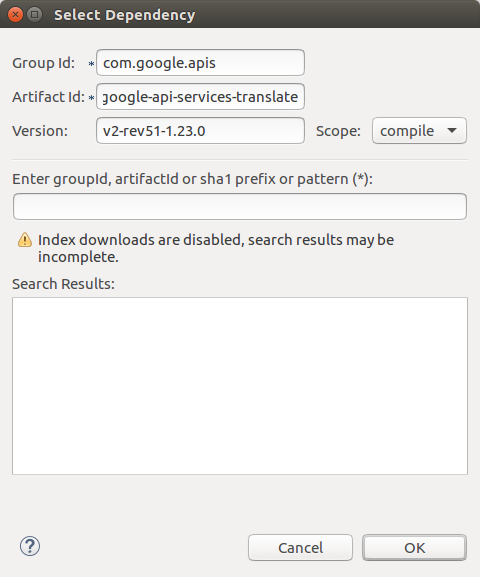
\includegraphics[width=\textwidth, keepaspectratio]{create-maven-project-3.png}
		\caption{Thêm Dependencies}
		\label{Them Dependencies}
	\end{figure}
	\end{item}
\end{enumerate}
\end{document}